\documentclass[a4paper,11pt]{article}

\usepackage[ansinew]{inputenc}
\usepackage[french]{babel}
\usepackage[T1]{fontenc}
\usepackage[paper=a4paper, top=1cm, bottom=1cm, left=2cm, right=2cm]{geometry}
\usepackage{graphicx}
\usepackage{hyperref}
\usepackage{url}
\usepackage{xcolor}

\title{\large{\bfseries{ARCHITECTURE LOGICIELLE}}}
\author{Benoît Védrenne, Gaël Walter}

\begin{document}

\maketitle

\begin{center}
\emph{Chargé de TD :} Damien Cassou\end{center}

\vspace{0.5cm}

\begin{center}

\includegraphics[width=2.5cm,height=2.5cm]{images/bdx1.eps}\\
\large{Université Bordeaux 1,\\
351 cours de la Libération,\\
33405 Talence Cedex,\\
France}
\end{center} 

\vspace{0cm}

\begin{center}
 \includegraphics[width=9cm,height=9cm]{images/zeldaNintendo.eps}
\end{center}

\begin{center}
 \large{The Cremi Legend Of Zelda}
\end{center}

\begin{abstract}
La légende raconte que la grande forêt d'Hyrule est occupée par Ganon, le
puissant Prince des Ténèbres. Ganon a capturé la fille du Roi qui tenta de séparer la
Triforce, puissant sortilège qui protège le royaume d'Hyrule. Ses guardes
maléfiques avancent à grand pas dans la forêt en détruisant tout sur leurs
passages\ldots \\
Il existe cependant un chevalier courageux, en ces temps de manants. 
On le reconnait facilement à sa chevelure blonde sous sa longue cape
verte. Apprenant la nouvelle de l'invasion, le regard noir,
il parti dans les haut bois de la forêt d'Hyrule pour les affronter tous et
libérer la fille du Roi nommée ``Zelda''.\\

The ``CREMI Legend of Zelda'', c'est l'histoire de ce jeune garçon, nommé
LinkAuber, alias Link qui doit sauver la princesse Zelda au péril de sa vie. \\
Une somme d'embûches l'attend. L'art de manier son épée pourra peut être
l'aider dans sa quête impossible: seul contre une armée entière.
\end{abstract}

\newpage

\section{Introduction}
Le framework de jeu plateforme dont nous disposions, nous a permis
d'implémenter une version du Jeu Zelda. Ce jeu, créé par Miyamoto (auteur
également de Donkey Kong et Mario), possède une version Nintendo de 1986. \\

Notre application s'inspire de cette version là, où l'on peut guider dans une
forêt le personnage Link. Il peut utiliser son épée avec la touche ``Espace'', comme notre version. \\
Nous l'avons bien sûr dénommé Cremi Legend Of Zelda car il a été principalement
développé au Cremi !

\subsection{Comment jouer à CLOZ ?}
Le but du jeu est de guider Link dans la forêt pour l'amener à Zelda avec les
touches fléchées. \\ 
On devra tout d'abord éliminer tout ses ennemis méléfiques en utilisant le coup
d'attaque par la touche ``Espace''. Ceux ci sont très énervés car
ils ont été prévenus de l'arrivé de Link, c'est pour cela qu'ils n'ont pas un
comportement très logiques. Parfois, il se peut qu'un ennemi plus robuste
surveille plus raisonnablement Zelda, il est donc plus difficile à tuer.\\

La difficulté du jeu réside dans le nombre d'ennemis à tuer, plus ou moins
forts selon leurs grades, mais aussi dans les différents objets
qui peuvent agrémenter le jeu. Le joueur est libre de tous les essayer.\\

La vie de Link démarre à ``100'' mais elle peut descendre très vite!

\subsection{Quelques règles du jeu}
Seul le clavier est utile au jeu, mais le menu permet d'autres actions.\\
Au croisement avec des ennemis, Link perd de la vie. S'il meurt, le niveau de
jeu redémarre au début. \\
Depuis le menu, on peut redémarrer la partie au début, mais aussi sauvegarder la
partie ou en restaurer une.\\
Lorsque tout les ennemis sont tués, il faut aller vers la princesse et le
niveau est gagné, on passe alors automatiquement au niveau suivant, s'il existe.
On peut trouver une arme sur le sol, Link peut attaquer avec. Il est possible
que certaines actions enlève cette arme. 

\subsection{Astuces}
Comme dans beaucoup de jeu vidéo d'aventure, nous avons laissé des codes
secrets que l'on peut chercher si l'on veut. Qu'il est agréable en étant joueur
de trouver ce genre de code!

\newpage

\section{Conception}

\subsection{Pacquetages}
Le paquetage ``\textbf{zelda}'' comprend plusieurs paquetages.\\
Le paquetage ``\textbf{base}'' permet de gérer l'interaction utilisateur, sons,
gestion de mouvements de personnages.\\ 
Le paquetage ``\textbf{rule}'' permet de
gérer les collisions ou blocages entre entités du jeu.\\ 
Le paquetage
``\textbf{level}'' permet de gérer la mise en place des niveaux du jeu, de la
lecture de fichier pour les niveaux, à la création de niveaux.\\ 
Le paquetage
``\textbf{game}'' contient les classes nécessaires à la création du jeu
(gestion de l'univers, sauvegarde de niveaux\ldots).\\ 
Le paquetage
``\textbf{observer}'' permet de gérer tout les observateurs du jeu.\\ 
Le paquetage ``\textbf{entity}'' possède toutes les classes de toutes les entités 
présentes dans le jeu : personnages et décors. Dans les personnages, un paquetage 
est réservé aux états de Link.\\

\subsection{Architecture générale}

\begin{center}
 %\includegraphics[width=9cm,height=9cm]{images/archiGenerale.eps}
\end{center}

\subsection{Architecture détaillée}

\subsubsection*{Une Fabrique Abstraite pour créer le niveau depuis un fichier
texte}
Nous avons choisi d'utilisé une fabrique abstraite pour permettre la
création et l'ajout d'entité dans le niveau. Il était assez interressant
de créer cette fabrique abstraite car aisni nous faisions juste une
demande de création d'un certain objet à celle-ci et elle s'occuper du
reste. Une personne voulant créer un personnage ou une autre entité a
juste besoin de faire appel à la méthode create adéquate. Cependant, le
problème le plus important et qui est un problème propre à ce modèle,
c'est que l'ajout de nouvelles entités est assez fastidieux.

\begin{center}
 %\includegraphics[width=9cm,height=9cm]{images/abstFab.eps}
\end{center}

\subsubsection*{Le pattern Monteur pour sauvegarder la partie}
Le fait de sauvegarder la partie est une action classique de tout
jeu. Il nous est apparu comme évident d'avoir une représentation sur
fichier du contenu de cette sauvegarde. Nous avons donc mis en place un
monteur, celui-ci en effet est particulièrement adapté à ce genre de
situation. Nous avons donc créer un monteur concret qui permet d'écrire
un fichier texte contenant les informations ainsi sauvegarder.\\
Un autre avantage de ce patron de conception est que nous pouvons ainsi
rapidement modifier la représentation de cette sauvegarde. Il est tout à
fait possible d'imaginé une sauvegarde au format HTML ou XML, ou on ne
sait quel autre format. Le format de la sauvegarde est donc facilement
modifiable pour n'importe quelle personne reprennant notre code et qui
n'aimerait pas notre représentation. \\

\begin{center}
 %\includegraphics[width=9cm,height=9cm]{images/monteur.eps}
\end{center}

Nous avons aussi utilisé ce modèle pour la lecture de la sauvegarde
ainsi que la lecture du fichier de création de niveau.

\subsubsection*{Gestion des états de Link avec le pattern Etat}
L'état de Link modifie son comportement. Ces changements
apparaissent de façon dynamique, selon les évenements du jeu, ou du joueur.
Cette intention nous a amené à utiliser le pattern Etat pour gérer Link. Celui
ci peut déléguer son comportement changeant à une hiérarchie de classes
LinkState possédant des requêtes spécifiques comme l'utilisation de l'arme, le
mode attaque, la mort du personnage\ldots
Sur la fin du développement, cette conception nous a permis de rajouter
rapidement de nouveaux états, et d'ajuster le comportement voulu facilement. \\

\begin{center}
 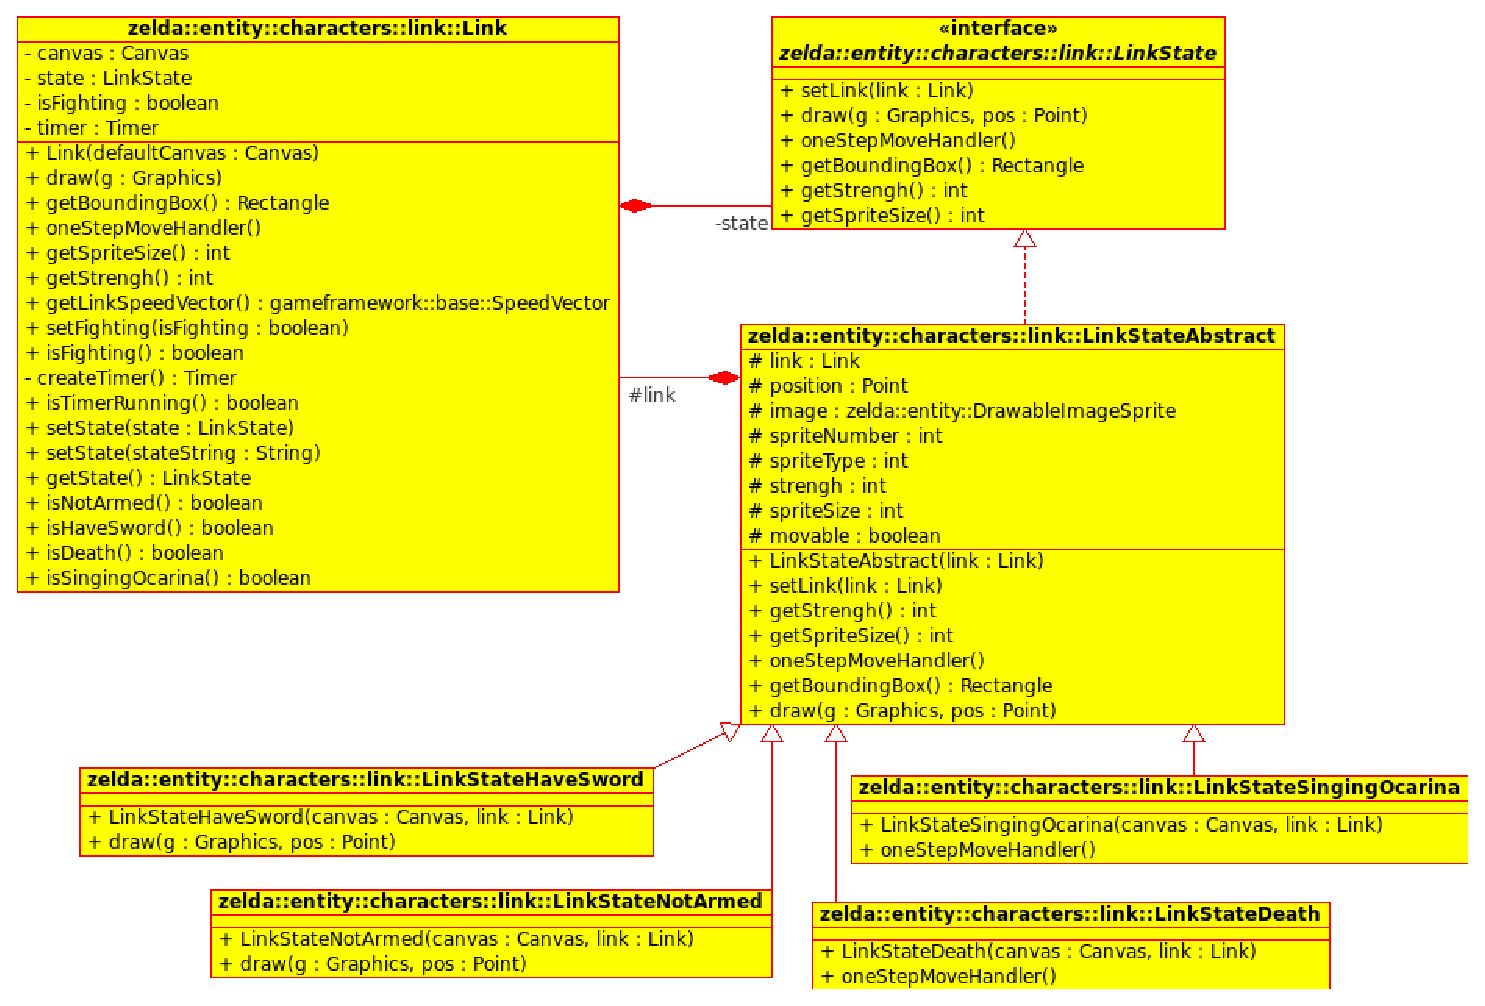
\includegraphics[scale=0.8]{images/Statediagram.eps}
\end{center}
 
\subsubsection*{Gestion du niveau avec des observateurs}
 
\end{document}
